\documentclass[a4paper,12pt]{article}

\usepackage[margin=0.75in]{geometry}
\usepackage[utf8]{inputenc}
\usepackage{t1enc}
\usepackage{lmodern}

\usepackage{xsim}
\usepackage{tasks}
\usepackage{animate}
\usepackage{caption}

\DeclareExerciseTranslation{magyar}{exercise}{feladat}
\DeclareExerciseEnvironmentTemplate{feladat}{
	{%
		\par\vspace{\baselineskip}
		\noindent
		\textbf{\GetExerciseProperty{counter}.~ \XSIMmixedcase{\GetExerciseName}}%
		\IfInsideSolutionF
		{
			\GetExercisePropertyT{subtitle}%
			{ {\normalfont\itshape\PropertyValue}}%
		}
	}
}
{}

\DeclareExerciseEnvironmentTemplate{megoldas}{
	{%
		\par\vspace{\baselineskip}
		\noindent
		\textbf{\XSIMmixedcase{\GetExerciseName}}%
		\IfInsideSolutionF
		{
			\GetExercisePropertyT{subtitle}%
			{ {\normalfont\itshape\PropertyValue}}%
		}
	}
}
{}
\xsimsetup{
	exercise/name=\XSIMtranslate{exercise},
	exercise/within=section,
	exercise/template=feladat,
	exercise/the-counter=\arabic{exercise},
	solution/name=megoldás,
	solution/print,
	solution/template=megoldas,
}

\usepackage[hungarian]{babel}
\usepackage{amsmath}
\usepackage{mathtools}
\usepackage{amsthm}
\usepackage{amsfonts}
\usepackage{amssymb}
\usepackage{graphicx}
\usepackage{wrapfig}
\graphicspath{{./images/}}
\usepackage{float}
\usepackage{multicol}

\usepackage{hyperref}
\hypersetup{
    colorlinks,
    citecolor=black,
    filecolor=black,
    linkcolor=black,
    urlcolor=black
}

\theoremstyle{definition}
\newtheorem{definition}{Definíció}
\newtheorem*{definition*}{Definíció}
\newtheorem*{remark}{Megjegyzés}
\newtheorem{theorem}{Tétel}
\newtheorem*{theorem*}{Tétel}
\newtheorem*{example}{Példa}
\newtheorem{notation}{Jelölés}
\newtheorem*{notation*}{Jelölés}

\usepackage{tikz}
\usetikzlibrary{automata,positioning}

\title{\huge{A számításelmélet alapjai} \\[-4pt] \large gyakorlati jegyzet \vspace{-15pt}}
\author{Boda Bálint}
\date{\vspace{-12pt}2023. tavaszi félév}

\DeclareMathOperator{\tr}{\delta}

\begin{document}
	\section{Automaták determinizálása}
	Alapötlet: hozzunk létre összevont állapotokat pl. az $ \left\lbrace q_1, q_2, q_3 \right\rbrace $ állapotot vonjuk össze a $ q_{123} $ állapottá. 
	\begin{example}
		Tekintsük a következő automatát:
		
		\begin{multicols}{2}
			\begin{figure}[H]
				\centering
				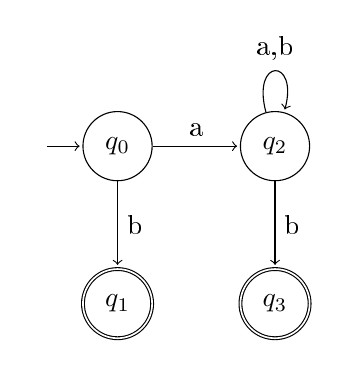
\begin{tikzpicture}[shorten >=1pt,node distance=2cm,on grid,auto] 
					\node[state,initial,initial text=] (q_0)   {$q_0$}; 
					\node[state, accepting] (q_1) [below =of q_0] {$q_1$}; 
					\node[state] (q_2) [right=of q_0] {$q_2$}; 
					\node[state,accepting](q_3) [below=of q_2] {$q_3$};
					\path[->] 
					(q_0) edge  node {b} (q_1)
					edge  node {a} (q_2)
					(q_2) edge [loop above] node {a,b} ()
					(q_2) edge  node {b} (q_3) ;
				\end{tikzpicture}
			\end{figure}
			\begin{table}[H]
				\centering
				$$
				\begin{array}{|c|c|c|}
					\hline
					& a & b \\
					\hline
					\rightarrow q_0 & \left\lbrace q_2 \right\rbrace & \left\lbrace q_1 \right\rbrace \\
					\hline
					q_1 & \varnothing  &  \varnothing \\
					\hline
					\leftarrow q_2 & \left\lbrace q_2 \right\rbrace & \left\lbrace q_2, q_3 \right\rbrace   \\
					\hline
					\leftarrow q_3 & \varnothing  & \varnothing \\
					\hline
				\end{array}
			$$
			\end{table}
		\end{multicols}
		\begin{remark}
			A nemdeterminisztikus automaták esetében a táblázatban gyakran egyelemű állapothalmazok helyett csak magát az állapotot írjuk le.
		\end{remark}
		\noindent
		Világos hogy az automata nem determinisztikus, ezért determinizáljuk: Az $q_0$ és $q_1$ sorokat változatlanul leírjuk a $q_2$ sorban azonban el kell végeznünk a $q_2$ és a $q_3$ összevonását.
		\begin{table}[H]
			\centering
			$$
			\begin{array}{|c|c|c|}
				\hline
				& a & b \\
				\hline
				\rightarrow q_0 &  q_2 & q_1 \\
				\hline
				q_1 & \varnothing  &  \varnothing \\
				\hline
				\leftarrow q_2 & q_2 & q_{23}    \\
				\hline
				\leftarrow q_3 & \varnothing  & \varnothing \\
				\hline
				? q_{23}& ? & ? \\
				\hline
			\end{array}
			$$
		\end{table}
		\noindent
		Mivel $q_2$ és $q_3$ közül legalább az egyik elfogadó állapot volt így az összevont állapot is elfogadó lesz. Ezt követően már csak az összevonásokat kell elvégeznünk:
		\begin{enumerate}
			\item $ \tr{(q_{23}, a)} = \tr{(q_2, a)} \, \cup \, \tr{(q_3, a)} = \left\lbrace q_2 \right\rbrace \, \cup \, \varnothing = \left\lbrace q_2 \right\rbrace \quad \text{Egyelemű, nem kell további összevonás} $
			\item $ \tr{(q_{23}, b)} = \tr{(q_2, b)} \, \cup \, \tr{(q_3, b)} = \left\lbrace q_{23} \right\rbrace \, \cup \, \varnothing = \left\lbrace q_{23} \right\rbrace \quad \text{Egyelemű, nem kell további összevonás} $
		\end{enumerate}
		\noindent
		Így az automata:
		
		\begin{multicols}{2}
			\begin{table}[H]
				\centering
				$$
				\begin{array}{|c|c|c|}
					\hline
					& a & b \\
					\hline
					\rightarrow q_0 & q_2  & q_1 \\
					\hline
					q_1 & \varnothing  &  \varnothing \\
					\hline
					\leftarrow q_2 & q_2 & q_{23}   \\
					\hline
					\leftarrow q_3 & \varnothing  & \varnothing \\
					\hline
					\leftarrow q_{23} & q_2 & q_{23} \\
					\hline
				\end{array}
				$$
			\end{table}
			\begin{figure}[H]
				\centering
				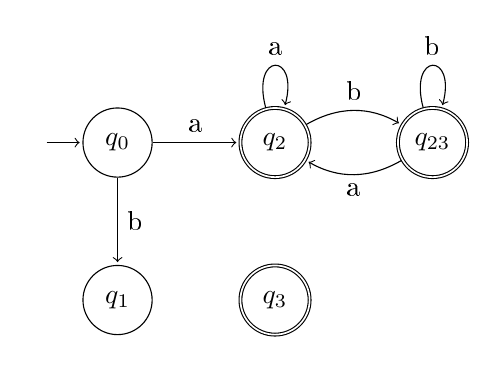
\begin{tikzpicture}[shorten >=1pt,node distance=2cm,on grid,auto] 
					\node[state,initial,initial text=] (q_0)   {$q_0$}; 
					\node[state] (q_1) [below =of q_0] {$q_1$}; 
					\node[state, accepting] (q_2) [right=of q_0] {$q_2$}; 
					\node[state,accepting](q_3) [below=of q_2] {$q_3$};
					\node[state,accepting](q_23) [right=of q_2] {$q_{23}$};
					\path[->] 
					(q_0) edge  node {b} (q_1)
					edge  node {a} (q_2)
					(q_2) edge [loop above] node {a} ()
					(q_2) edge [bend left] node {b} (q_23)
					(q_23) edge [bend left]  node {a} (q_2)
					(q_23) edge [loop above] node {b} ();
				\end{tikzpicture}
			\end{figure}
		\end{multicols}
		Észrevehetjük, hogy a $q_3$ állapot elérhetetlenné vált, azaz az automata elvesztette összefüggőségét. Az összefüggőség megőrzéséhez bevezethetünk egy egyszerű változtatást az algoritmusba, hogy egy sort állapotot csak akkor veszünk az új automatához, ha arra egy korábbi sor már hivatkozik.
	\end{example}
	\newpage
	\noindent
	Tekintsünk egy bonyolultabb példát:
	\begin{example}
	Determinizáljuk a következő automatát az optimalizált algoritmus alapján!
	\begin{table}[H]
		\centering
		$$
		\begin{array}{|c|c|c|}
			\hline
			& a & b \\
			\hline
			\rightarrow q_0 & \left\lbrace q_1, q_2 \right\rbrace & \varnothing \\
			\hline
			\leftarrow q_1 & q_1 &  q_2 \\
			\hline
			\leftarrow q_2 & q_0 & q_1   \\
			\hline
			q_3 & \left\lbrace q_1, q_3 \right\rbrace  & q_0 \\
			\hline
		\end{array}
		$$
	\end{table}
	\begin{enumerate}
		\item $ \tr(q_0,a) $ állapotokat össze kell vonni ($ q_{12} $)
		
		\item Meg kell határozni a $q_{12}$ sort:
		\begin{enumerate}
			\item $ \tr(q_{12},a) = \tr(q_{1},a) \cup \tr(q_{2},a) = q_{01} $
			\item $ \tr(q_{12},b) = \tr(q_{1},b) \cup \tr(q_{2},b) = q_{12} $
		\end{enumerate}
	
		\item Meg kell határozni a $q_{01}$ sort:
		\begin{enumerate}
			\item $ \tr(q_{01},a) = \tr(q_{0},a) \cup \tr(q_{1},a) = q_{12} \cup q_{1} =  q_{12} $
			\item $ \tr(q_{01},b) = \tr(q_{0},b) \cup \tr(q_{1},b) = q_{2} $
		\end{enumerate}
	
		\item Meg kell határozni a $q_{2}$ sort.
		\item Meg kell határozni a $q_{1}$ sort.
	\end{enumerate}
	\begin{table}[H]
		\centering
		$$
		\begin{array}{|c|c|c|}
			\hline
			& a & b \\
			\hline
			\rightarrow q_0 & q_{12} & \varnothing \\
			\hline
			\leftarrow q_{12} & q_{01} & q_{12}  \\
			\hline
			\leftarrow q_{01} & q_{12} & q_2   \\
			\hline
			\leftarrow q_{2} & q_0 & q_1   \\
			\hline
			\leftarrow q_{1} & q_1 & q_2   \\
			\hline
		\end{array}
		$$
	\end{table}
	Mivel minden állapot ismert az algoritmus optimalizált verziója véget ér.
	\end{example}
	
	\begin{example}
		Determinizáljuk a következő automatát az optimalizált algoritmus alapján!
		
		\begin{multicols}{2}
			\begin{table}[H]
				\centering
				$$
				\begin{array}{|c|c|c|}
					\hline
					& a & b \\
					\hline
					\rightarrow q_0 & \left\lbrace q_0, q_1 \right\rbrace  & \left\lbrace q_0, q_2 \right\rbrace  \\
					\hline
					q_1 & q_3 & \varnothing  \\
					\hline
					q_2 & \varnothing & q_4   \\
					\hline
					\leftarrow q_3 & q_3 & q_3   \\
					\hline
					\leftarrow q_4 & q_4 & q_4   \\
					\hline
				\end{array}
				$$
			\end{table}
			\begin{table}[H]
				\centering
				$$
				\begin{array}{|c|c|c|}
					\hline
					& a & b \\
					\hline
					\rightarrow q_0 & q_{01} & q_{02} \\
					\hline
					q_{01} & q_{013} & q_{02}  \\
					\hline
					q_{02} & q_{01} & q_{024}   \\
					\hline
					\leftarrow q_{013} & q_{013} & q_{023}   \\
					\hline
					\leftarrow q_{024} & q_{014} & q_{024}   \\
					\hline
					\leftarrow q_{023} & q_{013} & q_{0234}   \\
					\hline
					\leftarrow q_{014} & q_{0134} & q_{024}   \\
					\hline
					\leftarrow q_{0234} & q_{0134} & q_{0234}   \\
					\hline
					\leftarrow q_{0134} & q_{0134} & q_{0234}   \\
					\hline
				\end{array}
				$$
			\end{table}
		\end{multicols}
	\end{example}
	\newpage
	\section{Véges automaták összefüggővé alakítása}
	Egy automata összefüggő, ha minden állapot elérhető. Az összefüggővé alakítás algoritmusa a következő:
	\begin{itemize}
		\item $ H_0 = \left\lbrace q_0 \right\rbrace $
		\item $ H_{i+1} = H_i \cup \left\lbrace H_i \text{ valamely eleméből elérhető állapotok} \right\rbrace $ 
	\end{itemize}
	Az algoritmus akkor áll meg, ha $ H_{i+1} = H_i $. Az automata összefüggő, ha $ Q = H $. Az automata összefüggővé alakítható ha lecseréljük $ Q $-t $Q \cap H$-ra.
	\section{A 3-as normálforma}
	\begin{definition*}
		Egy $ G = (N, \Sigma, P, S) $ reguláris grammatikát hármas normálformájúnak (3NF) nevezünk, ha
		\[
		\forall p \in P \text{ produkciós szabályra igaz, hogy } A \rightarrow aB \text{ vagy } A \rightarrow \varepsilon \text{ alakú} \; \left( A,B \in N, a \in \Sigma \right) 
		\]
	\end{definition*}
	\subsection{3NF-re hozás}
	\begin{enumerate}
		\item Ellenőrzés, hogy a nyelv valóban reguláris-e
		\item Hossz redukció ($ A \rightarrow a_1,\dots,a_nB $ alakú szabályok felbontása)
		\item Láncmentesítés
		\begin{enumerate}
			\item Láncszabályok ($ A \rightarrow B $ alakúak) felírása
			\item $U$ halmazok meghatározása
			\item szabályhalmaz átalakítása
		\end{enumerate}
	\end{enumerate}
	\begin{example}
		Tekintsük a következő szabálykészletet:
		\[
		S \rightarrow abS \mid B, \quad B \rightarrow bB \mid V, \quad V \rightarrow aa \mid b
		\]
		\begin{enumerate}
			\item Hossz redukció:
			\begin{align*}
				S \rightarrow abS &\Rightarrow S \rightarrow aZ_1, \, Z_1 \rightarrow bS \\
				V \rightarrow aa &\Rightarrow V \rightarrow aZ_2, \, Z_2 \rightarrow aZ_3, \ Z_3 \rightarrow \varepsilon 
			\end{align*}
			Így az új szabálykészlet:
			\[
			S \rightarrow aZ_1 \mid B, \;
			Z_1 \rightarrow bS, \quad
			B \rightarrow bB \mid V, \quad
			V \rightarrow aZ_2, \;
			Z_2 \rightarrow aZ_3, \;
			Z_3 \rightarrow \varepsilon, \;
			V \rightarrow bZ_3
			\]
			\item Láncmentesítés: \\
			Láncszabályok: $ S \rightarrow B, \; B \rightarrow V $ \\
			$U$ halmazok:
			\begin{enumerate}
				\item $B$:
				\begin{align*}
					U_1(B) &= \left\lbrace B \right\rbrace \\
					U_2(B) &= U_1(B) \cup \left\lbrace \text{nemterminálisok melyekből } U_1(B) \text{ egyik eleme elérhető} \right\rbrace \\
					&= U_1(B) \cup \left\lbrace S \right\rbrace = \left\lbrace B, S \right\rbrace \\
					U_3(B) &= U_2(B) \cup \varnothing = \underline{\left\lbrace B, S \right\rbrace = U(B)}
				\end{align*}
				\item $V$:
				\begin{align*}
					U_1(V) &= \left\lbrace V \right\rbrace \\
					U_2(V) &= U_1(V) \cup \left\lbrace B \right\rbrace \\
					U_3(V) &= U_2(V) \cup \left\lbrace S \right\rbrace \\
					U_4(B) &= U_3(B) \cup \varnothing = \underline{\left\lbrace B, S, V \right\rbrace = U(V)}
				\end{align*}
	
			\end{enumerate}
			Szabályhalmaz átírása:
			\[
				S \rightarrow aZ_1 \mid bB \mid aZ_2 \mid bZ_3,  \;
				Z_1 \rightarrow bS, \quad
				B \rightarrow bB \mid aZ_2 \mid bZ_3 \quad
				Z_2 \rightarrow aZ_3, \;
				Z_3 \rightarrow \varepsilon
			\]
		\end{enumerate}
	\end{example}
\end{document}